\section{Особенности архитектур задачников Programming Taskbook и Unix Taskbook}

Электронный задачник по программированию Unix Taskbook, разработанный Ли Шэнюем в рамках выполнения выпускной работы в 2022 году, использует ту же архитектуру, что и задачник Programming Taskbook. Она основана на применении динамических библиотек и позволяет расширять набор заданий без перекомпиляции ядра задачника. Каждая группа заданий реализуется в виде отдельной динамической библиотеки со стандартным набором функций, которые вызываются из ядра на различных этапах выполнения задания (основными этапами является этап инициализации, при котором генерируются исходные данные, передаваемые учебной программе, и этап итоговой проверки, на котором результаты, полученные программой, сравниваются с контрольными данными). Кроме того, в динамической библиотеке можно определить способ отображения на экране всей информации, связанной с заданием. 
Подобная расширяемая архитектура дает возможность разрабатывать задачи самого разного содержания, в том числе связанные с обработкой файлов и каталогов (которые автоматически создаются при инициализации задания) и с многопоточным программированием, что было также продемонстрировано в выпускной работе.
Близость архитектур задачников  Unix Taskbook и Programming Taskbook и их гибкость дает основания предполагать, что перенос уже имеющихся групп задач из задачника Programming Taskbook в задачник Unix Taskbook окажется не слишком сложным.
Все задачи, входящие в задачник Programming Taskbook, подготовлены на основе конструктора учебных заданий TaskMaker, содержащего набор функций для генерации формулировок заданий, исходных и контрольных данных, настройки их отображения на экране, задания дополнительных свойств конкретной задачи (например, количества необходимых тестовых испытаний учебной программы). Конструктор TaskMaker реализован для нескольких языков (Pascal, C++, C\#, PascalABC.NET), однако базовый набор из 1100 задач реализован на языке Pascal в среде Delphi (в которой было первоначально реализовано и ядро задачника Programming Taskbook).
В то же время, задачник Unix Taskbook реализован на языке C++; именно это позволяет легко адаптировать его к различным операционным системам на базе Unix. Поэтому необходимо разработать механизм, который дал возможность переносить задания из базового набора (а также расширений) задачника Programming Taskbook в задачник Unix Taskbook без переписывания кода, связанного с генерацией заданий.


\begin{figure}[htbp]%
    \centering
    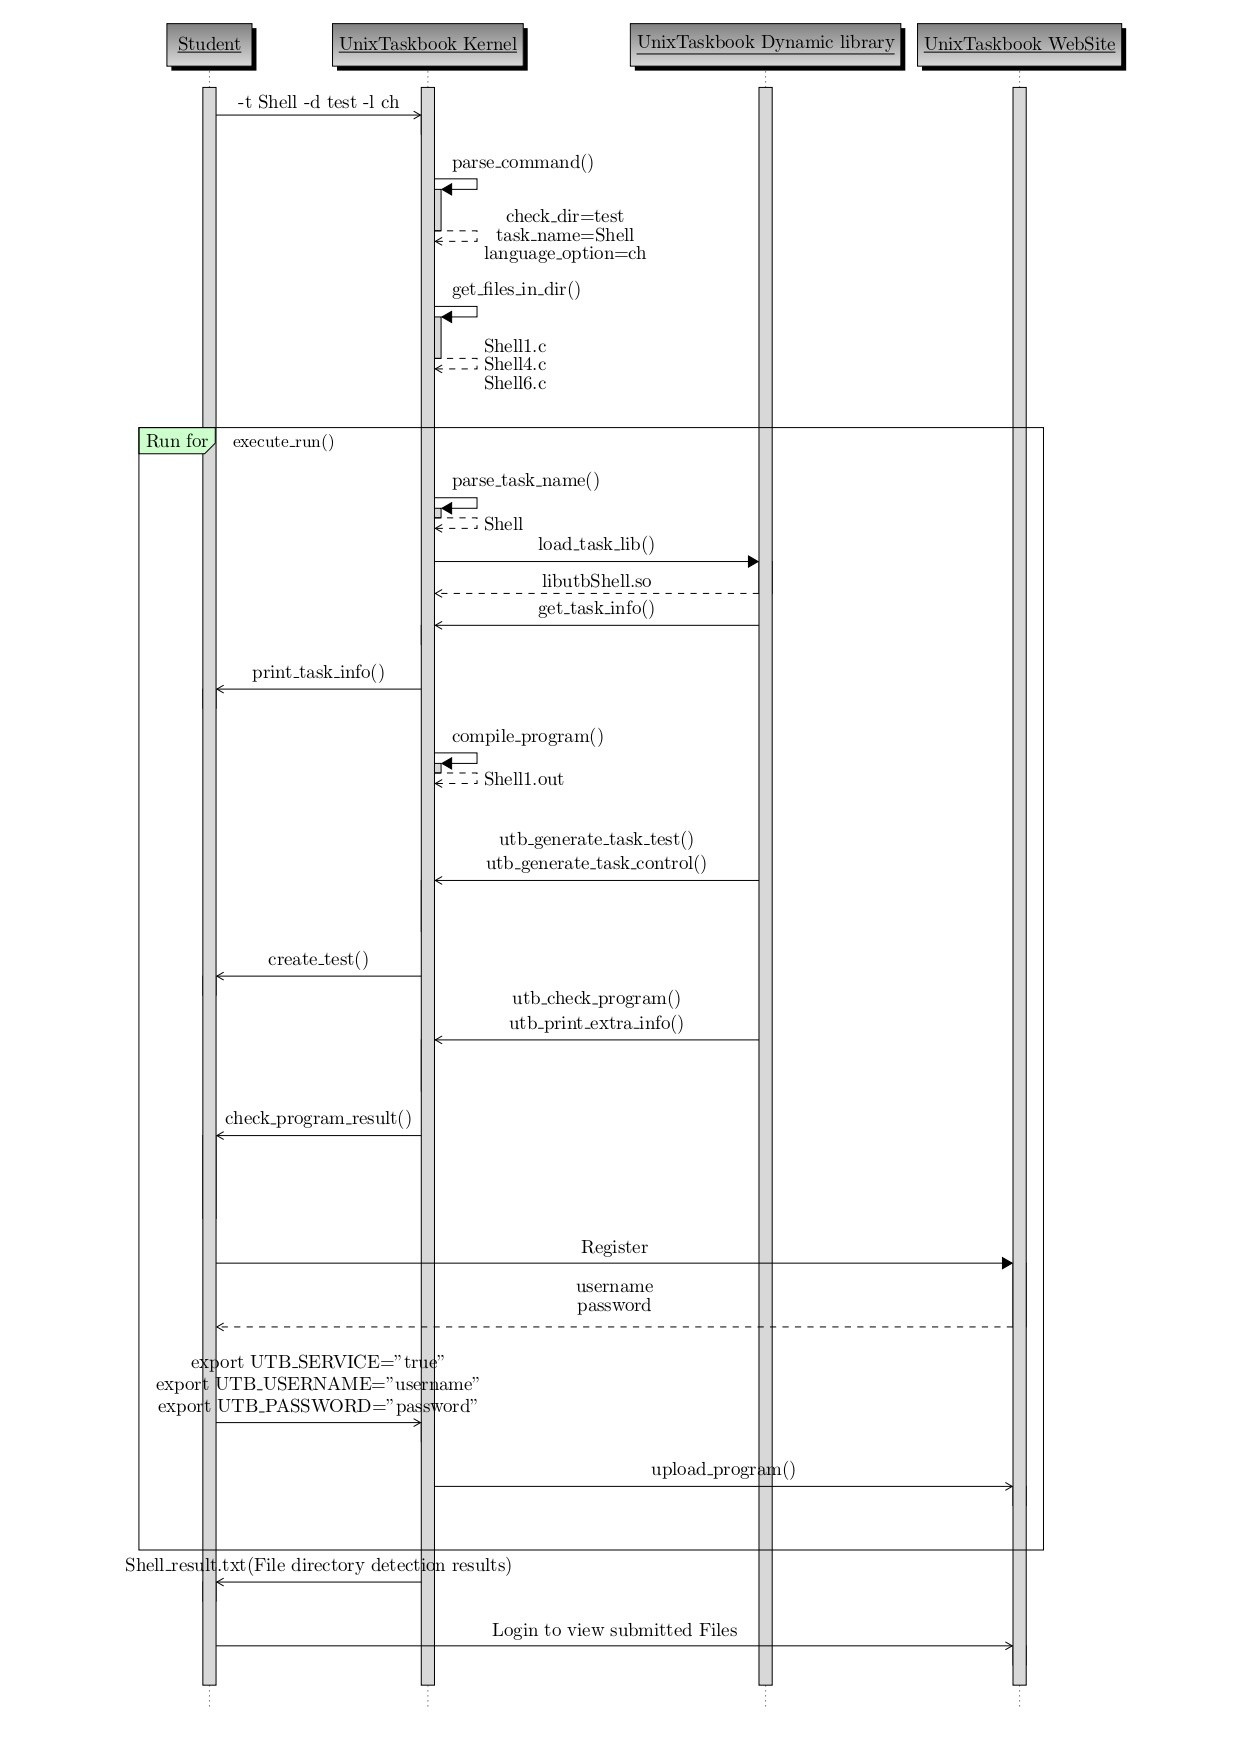
\includegraphics[width=0.68\linewidth]{images/utb.jpg}%子图文件名
    \caption{архитектур Unix Taskbook\cite{ref20}}%总标题
    \label{utb}%总标签
\end{figure}

\newpage